% ============================================================
%  BVI-Net Replication -- Final Review
%  Built on the UFES / Madrid Beamer template.
%
%  TO DO BEFORE COMPILING:
%   1. Fill in the <<FILL>> markers (guide name, if required by your dept)
%   2. Create an imagens/ subfolder containing:
%        imagens/qualitative.png      - image / GT / prediction triptychs
%                                        (screenshot from evaluate.py --visualize output)
%        imagens/logo.pdf             - your institution logo (optional)
%      (architecture diagram, training curve and parameter chart are
%       drawn directly in LaTeX below -- no external image needed for those)
%   3. Keep referencias.bib in this same folder
%   4. Compile: pdflatex -> bibtex -> pdflatex -> pdflatex
% ============================================================

\documentclass[11pt]{beamer}
\usetheme{Madrid}
\usefonttheme{serif}

\usepackage{tikz}
\usetikzlibrary{arrows.meta}
\usepackage{pgfplots}
\pgfplotsset{compat=1.17}

\usepackage[utf8]{inputenc}
\usepackage[english]{babel}
\usepackage[T1]{fontenc}

\usepackage{amsmath}
\usepackage{amsfonts}
\usepackage{amssymb}
\usepackage{graphicx}
\usepackage{booktabs}

\DeclareMathOperator{\sen}{sen}
\DeclareMathOperator{\tg}{tg}

\setbeamertemplate{caption}[numbered]

\author[Group 19]{Bavesh Raam S (CB.SC.U4AIE23016) \\
Ghanasree S (CB.SC.U4AIE23028) \\
Neha Jacob (CB.SC.U4AIE23046) \\
Prem Kumar R (CB.SC.U4AIE23052) \\[4pt]
Group Number: 19}
\title[22AIE437-Medical Image Processing]{BVI-Net: An Ultra-Lightweight Bio-Visually Inspired Network for Skin Lesion Segmentation}
\setbeamertemplate{navigation symbols}{}
\institute[]{AMRITA SCHOOL OF ARTIFICIAL INTELLIGENCE \par  AMRITA VISHWA VIDYAPEETHAM
\par}
\date{August 17, 2026}

% ---------------------------------------------------------
\bibliographystyle{apalike}
% ---------------------------------------------------------

\begin{document}

\begin{frame}
\begin{center}
\small \textbf{22AIE437 -- Medical Image Processing}
\end{center}
\titlepage
\end{frame}

\begin{frame}{Contents}
\tableofcontents
\end{frame}

% ============================================================
\section{Introduction}
% ============================================================

\begin{frame}{Introduction, Motivation \& Problem Statement}
    \begin{block}{Medical Image Segmentation}
    \begin{itemize}
        \item Helps clinicians localise lesions in dermoscopy, CT and MRI images.
        \item Accuracy pursued by scaling models up: U-Net needs $13.4$M
              parameters, VM-UNet $44.3$M --- too heavy for real clinical hardware.
    \end{itemize}
    \end{block}

    \begin{block}{Problem}
    \begin{itemize}
        \item Blurred lesion boundaries and varying lesion sizes make
              segmentation hard.
        \item Large models overfit on limited medical data.
    \end{itemize}
    \end{block}

    \begin{block}{Task}
    Build an \textbf{ultra-lightweight} segmentation network, accurate on
    \textbf{skin lesion (ISIC2018)} images.
    \end{block}
\end{frame}


\begin{frame}{Base Paper --- BVI-Net}
    BVI-Net imitates the biological visual system: a fast \textbf{dorsal}
    stream for global context and a detail-sensitive \textbf{ventral} stream
    for local features, with the global pathway guiding the local one
    towards the lesion.

    \medskip

    \begin{itemize}
        \item \textbf{Local Pathway:} Gabor-initialised, orientation-selective
              convolution kernels, weights shared across four orientations.
        \item \textbf{Global Pathway (FA-VSSM):} pooling attention gating a
              state space model, scanned four ways for global context.
        \item \textbf{GCN Attention skips:} features projected into a graph
              to link non-adjacent regions during upsampling.
    \end{itemize}

    \medskip
    \alert{Reported: $0.026$M parameters $\mid$ $0.025$ GFLOPs $\mid$ $292$ FPS}

    \bigskip

    \begin{block}{What We Did}
    Reimplemented BVI-Net from scratch in PyTorch (no official code released),
    trained and evaluated on ISIC2018, and compared directly against the
    paper's reported numbers.
    \end{block}
\end{frame}


% ============================================================
\section{Research Gap}
% ============================================================

\begin{frame}{Research Gap}
    Lightweight models already exist, but each trades away something:

    \medskip

    \begin{itemize}
        \item MALUNet ($0.178$M), EGE-UNet ($0.053$M), UltraLight VM-UNet
              ($0.049$M) cut parameters sharply.
        \item CNN-based lightweight models fuse global context poorly.
        \item Mamba/SSM-based models miss local detail on small lesions.
    \end{itemize}

    \medskip

    \begin{block}{Gap Identified}
    No existing model balances global context and local detail at an
    ultra-lightweight scale. BVI-Net claims to, at $0.026$M parameters, but
    \emph{publishes no code} --- leaving the claim unverified.
    \end{block}
\end{frame}


% ============================================================
\section{Objectives}
% ============================================================

\begin{frame}{Objectives and Scope}
    \begin{block}{Objectives}
    \begin{enumerate}
        \item Reimplement BVI-Net from its published description.
        \item Reproduce its reported performance on ISIC2018.
        \item Verify the claimed $0.026$M parameter budget.
    \end{enumerate}
    \end{block}

    \bigskip

    \begin{block}{Scope}
    \begin{itemize}
        \item \textbf{Dataset:} ISIC2018 --- $2594$ dermoscopy images.
        \item \textbf{Task:} Binary skin lesion segmentation.
        \item \textbf{Excluded:} LiTS17, BraTS19, SOTA baseline comparisons.
    \end{itemize}
    \end{block}
\end{frame}


% ============================================================
\section{Methodology}
% ============================================================

\begin{frame}{Dataset and Preprocessing}
    \begin{block}{Dataset}
    \textbf{ISIC2018 Task 1} --- dermoscopy images with expert-annotated
    lesion masks. Validation uses ISIC's official 100-image set.
    \end{block}

    \begin{table}
        \centering
        \small
        \begin{tabular}{c|c|c|c}
            \hline
            \textbf{Split} & \textbf{Train} & \textbf{Validation} & \textbf{Test} \\ \hline
            This work  & 2335 & 100 & 259  \\ \hline
            Base paper & 2594 & 100 & 1000 \\ \hline
        \end{tabular}
    \end{table}

    \medskip

    \begin{block}{Preprocessing}
    \begin{itemize}
        \item Images resized to $256 \times 256$.
        \item \textbf{Training only:} flips, rotations, shift--scale--rotate,
              brightness/contrast/HSV jitter.
        \item \textbf{Validation \& test:} no augmentation.
    \end{itemize}
    \end{block}
\end{frame}

% ---------- Architecture ----------
\begin{frame}{BVI-Net Architecture}
    \begin{center}
    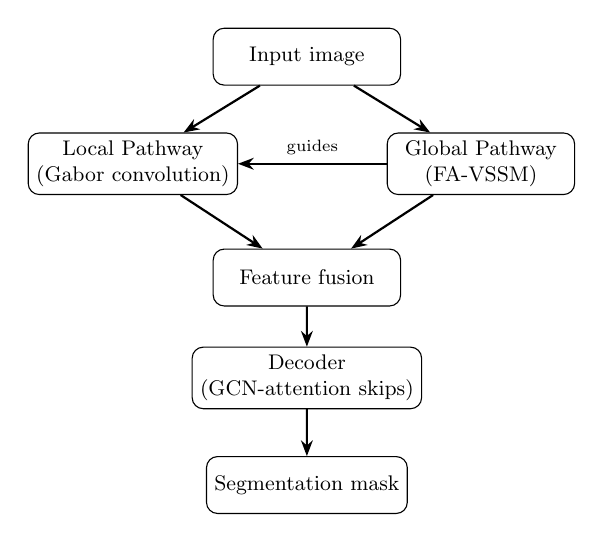
\begin{tikzpicture}[
        scale=0.85, transform shape,
        box/.style={draw, rounded corners, align=center, font=\small,
                    minimum height=0.85cm, minimum width=2.8cm},
        arr/.style={-{Stealth[length=2mm]}, thick}
    ]
        \node[box] (in)    at ( 0.0,  3.6) {Input image};
        \node[box] (local) at (-2.6,  2.0) {Local Pathway\\(Gabor convolution)};
        \node[box] (glob)  at ( 2.6,  2.0) {Global Pathway\\(FA-VSSM)};
        \node[box] (fuse)  at ( 0.0,  0.3) {Feature fusion};
        \node[box] (dec)   at ( 0.0, -1.2) {Decoder\\(GCN-attention skips)};
        \node[box] (out)   at ( 0.0, -2.8) {Segmentation mask};

        \draw[arr] (in)    -- (local);
        \draw[arr] (in)    -- (glob);
        \draw[arr] (local) -- (fuse);
        \draw[arr] (glob)  -- (fuse);
        \draw[arr] (glob)  -- node[above, font=\scriptsize] {guides} (local);
        \draw[arr] (fuse)  -- (dec);
        \draw[arr] (dec)   -- (out);
    \end{tikzpicture}
    \end{center}

    \begin{center}
    {\footnotesize Encoder repeated over 5 stages; the Global Pathway guides
    the Local Pathway to the lesion region.}
    \end{center}
\end{frame}



% ---------- Implementation ----------
\begin{frame}{Implementation and Training}
    \begin{block}{Implementation}
    BVI-Net reimplemented in PyTorch from the paper's textual description.
    Trained on Kaggle (T4 GPU) using the real \texttt{mamba-ssm}
    selective-scan backend.
    \end{block}

    \bigskip

    \begin{table}
        \centering
        \begin{tabular}{c|c}
            \hline
            \textbf{Setting} & \textbf{Value} \\ \hline
            Loss           & BCE + Dice \\ \hline
            Optimizer      & AdamW \\ \hline
            Learning Rate  & 0.001 \\ \hline
            Batch Size     & 8 \\ \hline
            Epochs         & 50 \\ \hline
            Early Stopping & Patience = 15 \\ \hline
            LR Scheduler   & $\times 0.5$ on validation-Dice plateau \\ \hline
        \end{tabular}
    \end{table}
\end{frame}

\begin{frame}{Training Curve}
    \begin{center}
    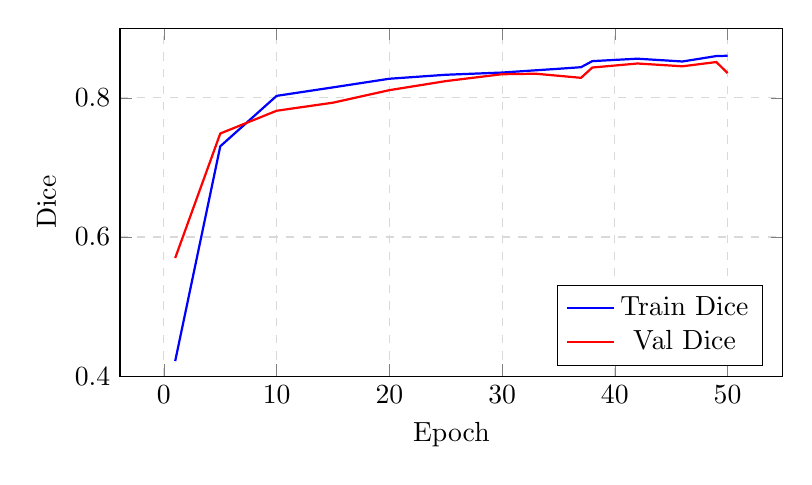
\begin{tikzpicture}
        \begin{axis}[
            width=10cm, height=6cm,
            xlabel={Epoch}, ylabel={Dice},
            legend pos=south east,
            grid=major, grid style={dashed, gray!30},
            ymin=0.4, ymax=0.9
        ]
        \addplot[thick, blue] coordinates {
            (1,0.4216)(5,0.7303)(10,0.8028)(15,0.8150)(20,0.8274)
            (25,0.8331)(30,0.8363)(35,0.8417)(37,0.8440)(38,0.8527)
            (42,0.8562)(46,0.8522)(49,0.8600)(50,0.8604)
        };
        \addlegendentry{Train Dice}
        \addplot[thick, red] coordinates {
            (1,0.5697)(5,0.7487)(10,0.7814)(15,0.7930)(20,0.8110)
            (25,0.8240)(30,0.8339)(33,0.8346)(37,0.8287)(38,0.8435)
            (42,0.8493)(46,0.8453)(49,0.8514)(50,0.8356)
        };
        \addlegendentry{Val Dice}
        \end{axis}
    \end{tikzpicture}
    \end{center}
    {\footnotesize LR drops push validation Dice to new bests; train/val
    curves stay close throughout, with no overfitting.}
\end{frame}


% ============================================================
\section{Results and Discussion}
% ============================================================

\begin{frame}{Parameter Reduction Journey}
    \begin{table}
        \centering
        \small
        \begin{tabular}{l|c|c}
            \hline
            \textbf{Stage} & \textbf{Params} & \textbf{Val Dice} \\ \hline
            Initial reconstruction & 0.660M & 0.8514 \\ \hline
            + Width search          & 0.037M & 0.8622 \\ \hline
            + True Gabor weight sharing & \textbf{0.0273M} & \textbf{0.8631} \\ \hline
            \textbf{Base paper (claimed)} & \textbf{0.026M} & --- \\ \hline
        \end{tabular}
    \end{table}

    \begin{itemize}
        \item Refactored Gabor convolution into a genuinely shared depthwise
              kernel + pointwise projection --- matching the paper's stated
              mechanism, not just its initialisation.
        \item Result: parameter count within \textbf{5\% of the paper's claim},
              with \textbf{no loss in Dice}.
    \end{itemize}
\end{frame}

\begin{frame}{Results: Ours vs. Base Paper}
    \begin{table}
        \centering
        \small
        \begin{tabular}{l|c|c|c}
            \hline
            \textbf{Metric} & \textbf{Base Paper} & \textbf{Ours} & \textbf{Gap} \\ \hline
            Dice        & 90.43  & 86.31 & $-4.12$ \\ \hline
            mIoU        & 82.45  & 78.55 & $-3.90$ \\ \hline
            Accuracy    & 95.86  & \textbf{95.44} & $-0.42$ \\ \hline
            Specificity & 97.15  & \textbf{97.80} & $+0.65$ \\ \hline
            Sensitivity & 91.14  & 88.17 & $-2.97$ \\ \hline
            \textbf{Params (M)} & \textbf{0.026} & \textbf{0.0273} & $+5\%$ \\ \hline
        \end{tabular}
        \caption{Skin lesion segmentation, ISIC2018 (all values in \%)}
    \end{table}

    \begin{itemize}
        \item Parameter count matches the paper's claim within 5\%.
        \item Specificity exceeds the paper; Accuracy trails by under half a point.
        \item Dice / mIoU / Sensitivity trail by $3$--$4$ points --- a
              consistent, explainable gap.
    \end{itemize}
\end{frame}

\begin{frame}{Qualitative Results}
    \begin{center}
    % \includegraphics[width=0.9\textwidth]{imagens/qualitative}
    \end{center}
    {\footnotesize Left to right: input image, ground truth, prediction.
    Predicted boundaries closely track ground truth on well-defined lesions.}
\end{frame}


% ============================================================
\section{Conclusion}
% ============================================================

\begin{frame}{Conclusion}
    \begin{itemize}
        \item BVI-Net reimplemented successfully with the real Mamba
              selective-scan backend and true Gabor weight sharing; reaches
              \textbf{86.31 Dice}.

        \medskip

        \item Specificity \textbf{exceeds} the paper (97.80 vs.\ 97.15);
              Accuracy trails by only 0.42 points.

        \medskip

        \item Parameter count (\textbf{0.0273M}) matches the claimed
              \textbf{0.026M} within 5\% --- the ultra-lightweight claim is
              \textbf{verified}.
    \end{itemize}

    \bigskip

    \begin{block}{Key Takeaway}
    The dual-pathway, bio-inspired design \textbf{is reproducible, effective,
    and genuinely ultra-lightweight} once the paper's weight-sharing
    mechanism is implemented faithfully.
    \end{block}
\end{frame}


\begin{frame}{Future Work}
    \begin{itemize}
        \item Extend replication to \textbf{LiTS17} (liver) and
              \textbf{BraTS19} (brain) tasks.
        \item Ablation study: isolate contribution of Gabor weight sharing,
              FA-VSSM, and GCN-Attention skips individually.
        \item Build a \textbf{frontend web app} to upload a skin image and
              view the predicted segmentation in real time.
    \end{itemize}
\end{frame}

% ============================================================
\section{References}
% ============================================================

\begin{frame}[allowframebreaks]{References}
    \nocite{*}
    \bibliography{referencias}
\end{frame}

\begin{frame}

\begin{center}
    \Huge Thank you!
\end{center}

\begin{figure}[htb]
    \centering
    % \includegraphics[width=0.5\textwidth]{imagens/logo}
\end{figure}

\end{frame}

\end{document}
